\documentclass[tikz]{standalone} 
\usetikzlibrary{matrix}
\begin{document}

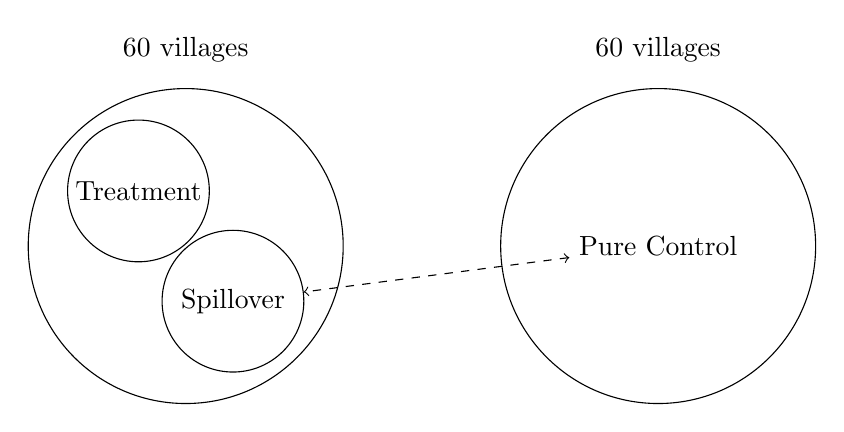
\begin{tikzpicture} 
\draw (0,0) circle [radius=2cm];
%\foreach \i [count=\j] in {18,36,...,360}
%  \draw (0,0)--(\i:2cm) node[shift=(\i:1em)]{\small\j}; 
\draw (6,0) circle [radius=2cm];
\node[] at (0,2.5) {60 villages};
\node[] at (6,2.5) {60 villages};
\node[] at (6,0) (A) {Pure Control};
\node[draw,circle,minimum size=1.8cm,inner sep=0pt] at (0.6,-0.7) (B) {Spillover};
\node[draw,circle,minimum size=1.8cm,inner sep=0pt] at (-0.6,0.7) {Treatment};
\draw [dashed,<->] (A) -- (B);
\end{tikzpicture} 

\end{document}